\documentclass[12pt]{report}

\usepackage[top=2cm,bottom=2cm,left=2cm,right=2cm]{geometry}
\usepackage[pdftex]{graphicx} 
\usepackage[utf8]{inputenc}   
\usepackage[english]{babel}
\usepackage{amsthm}
\usepackage{dsfont} % for the R of real
\usepackage{physics}
\usepackage{bm} % for a textbf in math mode

\theoremstyle{plain}
\newtheorem{THEO}{Theorem}
\newtheorem{DEF}{Definition}
\newtheorem{PROP}{Proposition}
\newtheorem{LEM}{Lemma}
\newtheorem{EX}{Example}
\newtheorem{COR}{Corollary}

\newcommand\mcl[1]{\mathcal{#1}}

\begin{document}
\begin{flushleft}
	
	\begin{center}
		\begin{figure}
			\centering
			
\includegraphics[scale=.13]{images/logo_unipd.png}
		\end{figure}
		Università degli studi di Padova\\
		Dipartimento di Fisica “Galileo Galilei”\\
		Academic year 2019/2020\\

		\vspace{1cm}		
		\large{\textit{Master degree in Physics of Data}}\\
		\vspace{1cm}
		\huge{\textbf{Notes of Machine Learning}}
	\end{center}
	
\tableofcontents


\chapter*{What is Machine Learning?}
The main subject o these notes is automated learning, or, as we will more often call it, Machine Learning (ML). Machine Learning is essentially "teaching to the computers so they can learn from inputs we give them". The input to a learning algorithm is training data, representing experience, and the output is some expertise, usually a new program that can independently perform a task.\\
A tipical example of a learning algorithm is a program that can distnguish between male and female people: it will be trained with a sample of different people (more heterogeneous as possible) to teach it the main differences of the two genres.\\
Another example is an algorithm that gives the probability of a person to have a certain height given, for example, the genre or the age.\\
A more common example is the algorithm that, between emails, can distinguish spam emails from the other ones.\\
Before starting the effective lectures, we should define a first small difference between the types of learning: 
since learning involves an interaction between the learner and the environment, one can divide learning tasks according to the nature of that interaction.  
\begin{itemize}
\item \textit{Supervised learning} describes a scenario in which the "experience", the training data, contains significant information that is missing in the unseen “test examples” to which the learned expertise is to be applied. In this setting, the acquired expertise is aimed to predict that missing information for the test data. In such cases, we can think of the environment as a teacher that “supervises” the learner by providing the extra information (labels). More abstractly, the algorithm can be seen as a process of "using experience to gain experties".
\item In \textit{Unsupervised learning}, instead, there is no distinction between training and test data: the learner processes input data with the goal of coming up with some summary, or compressed version of that data.
\end{itemize}


\chapter{Machine Learning Model}

First of all, we give some definitions of the stuff the machine learnig algorithm has access to:
\begin{itemize}
\item \textbf{Domain set} (or \textbf{instance space} $\mcl{X}$): is the set of all possible objects that we want to label, i.e. make prediction about. Usually this is a "vector of features".
\item \textbf{Label set}: contains all possible prediction (labels). Usually correspond to the binary set $\left\{0,1\right\}$ (that can mean $\left\{True,False\right\}$).
\item \textbf{Training data}: $S=((x_1,y_1),\dots,(x_m,y_m))$ is a finite sequence of pairs in $\mcl{X}\times \mathcal{y}$, and represent the input of the ML algorithm. The index $m$, instead, represent the dimension of the dataset. Despite the "set" notation, $S$ is a sequence. In particular, the same example may appear twice in $S$ and some algorithms can take into account the order of examples in $S$.
\item \textbf{Prediction rule}: Is a function $h:\mcl{X}\to\mcl{y}$ (also called "predictor", "hypotheses" or "classifier") that can be used to predict the label of new domain points. We denote $A(S)$ the hypothesis that a learning algorithm $A$ returns upon receiving the training sequence $S$.
\item \textbf{Data-generation model}: We assume that the instances are generated by some probability distribution $\mcl{D}$ (not known by the algorithm), and we assume that there is a "correct" labelling function $f:\mcl{X}\to\mcl{y}$ for which $y_i = f(x_i) \quad \forall i$. The labelling function isn't known by the algorithm: in fact, it is just what the program is trying to figure out. In summary, each pair in the training data is generated by first sampling a point $x_i$ according to $\mcl{D}$ and then labelling it by $f$.
\item \textbf{Measure of success}: We define \textit{error of the classifier} the probability that the algorithm does not predict the correct label on a random data point generated by distribution $\mcl{D}$. In other words, the error of $h$ i the probability to draw a random instance $x$, according to the distribution $\mcl{D}$, such that $h(x) \neq f(x)$.
\end{itemize}

Usually, our sample will be a vector (so a set of numbers) $x\in\mathds{R}^d$.\\
We must pay attention that what the algorithm learn depends on training data! So, if the training data are bad, the results will be bad aswell.

\section{Measure of Success: Loss Function}

Given a domain subset $A\subset\mcl{X}$ and the probability distribution $\mcl{D}$, $\mcl{D}(A)$ represents the probability of observing a point $x\in A$.\\
In many cases, we refer to $A$ as an \textit{event} and express it using a function $\pi :\mcl{X}\to\left\{0,1\right\}$, that is $A = \left\{x\in\mcl{X}:\pi(x)=1\right\}$.\\   
In this case denote $\mcl{D}(A)$ as $\mathds{P}_{x\sim\mcl{D}}\left[\pi(x)\right]$, where $\sim$ indicates that $x$ point is sampled according to $\mcl{D}$.\\
Now, we define the \textbf{error of prediction rule}:
\begin{equation}
\ell_{\mcl{D},f}(h) = \ell_\mcl{D}(h) = \mathds{P}_{x\sim\mcl{D}}\left[h(x)\neq f(x)\right] = \mcl{D}\left(\left\{x:h(x)\neq f(x)\right\}\right)
\label{eq:err_pred_rule}
\end{equation}
This is nothing but the probability of randomly choosing an example $x$ for which $h(x)\neq f(x)$. It is also called \textit{generalization error}, or \textbf{true error}.\\
It is important to understand that the algorithm doesn't know the probability distribution $\mcl{D}$, so it is not able to compute the true error. 

\section{Empirical Risk Minimization}

As mentioned earlier, a learning algorithm receives as input a training set $S$, sampled from an unknown distribution $\mcl{D}$ and labeled by some target function $f$, and should output a predictor $h_S:\mcl{X}\to\mcl{Y}$ (the subscript $S$ emphasizes the fact that the output predictor depends on the training set). The goal of the algorithm is to find $h_S$ that minimizes the error with respect to the unknown $\mcl{D}$ and $f$.\\
If, because of the true error can't be computed, we would like to try another estimate of it, we should define the error on the training data, called \textbf{training error}:
\begin{equation}
\ell_S(h) = \frac{\abs{i:h(x_i)\neq y_i , i=1,\dots ,m}}{m}
\label{eq:train_err}
\end{equation}
This division is simply the rate o correct prediction and the total samples (assuming classification problem and 0-1 loss), and it is also called \textit{empirical error} or \textit{empirical risk}.\\
This learning paradigm, which main goal is to find a predictor $h$ that minimize $\ell_S$, is called \textit{Empirical Risk Minimization} or ERM, for short.\\

\vspace{0.5cm}
Although the ERM rule seems very natural, without being careful this approach may fail miserabily.\\
Let's consider, for example, the sample in figure \ref{fig:overfit} (on the left), assuming a probability distribution $\mcl{D}$ for which instances $x$ are taken uniformily at random in the square, and the labelling function $f$ that assign the value 1 to the instances in the upper squares, and 0 to the others (essentially 0 to blue ones and 1 to red ones). If we collect the training set shown in figure \ref{fig:overfit} (on the right), to train the ML algorithm, a good predictor seems to be the function $h_S(x) = \left\{\begin{aligned} &0 \text{ if x in left side}\\ &1 \text{ if x in right side}\end{aligned}\right.$, that effectively minimize the training loss ($L_S(h_S) =0$, practically perfect). But is this a good predictor?

\begin{figure}[hbtp]
\centering
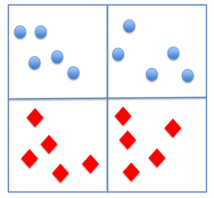
\includegraphics[scale=1.5]{images/overfit_ex_1.pdf}\qquad\qquad
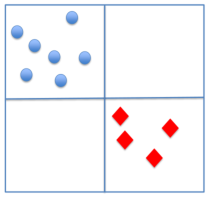
\includegraphics[scale=1.5]{images/overfit_ex_2.pdf}
\caption{Example of overfitting}
\label{fig:overfit}
\end{figure}

On the other hand, the true error of any classifier is, in this case $L_\mcl{D}(h_S) = \frac{1}{2}$.\\
We have found a predictor whose performance on the training set is excellent, yet its performance on the true “world” is very poor. This phenomenon is called overfitting. Intuitively, overfitting occurs when our hypothesis fits the training data “too well”, but doesn't have the same performances on a generic dataset. We obviously want to avoid this overfitting, because algorithms should work in general cases. Overfitting is less probable when the training set is large. The bigger is a training set, the smaller will be the probability to have regular distribution of data.\\


\section{Hypothesis class}
Rather than giving up completely the ERM paradigm, we want to look at the conditions under which it is guarantee that ERM does not overfit.\\
A common solution is to apply the ERM learning rule over a restricted search space. Formally, the learner should choose in advance (before seeing the data) a set of predictors. This set is called a \textbf{hypothesis class} and is denoted by $\mcl{H}$. Each $h\in\mcl{H}$ is a function mapping from $\mcl{X}$ to $\mcl{Y}$. For a given class $\mcl{H}$, and a training sample, $S$, the $ERM_\mcl{H}$ learner uses the ERM rule to choose a predictor $h$, with the lowest possible error over $S$:
\begin{equation}
ERM_\mcl{H} \in \underset{h\in\mcl{H`}}{argmin}\, L_S(h)
\label{eq:ERMH}
\end{equation}
where $argmin$ stands for the set of hypotheses in $\mcl{H}$ that achieve the minimum value of $L_S(h)$.\\
Since the choice of such a restriction is determined before the learner sees the training data, it should ideally be based on some prior knowledge about the problem to be learned. Intuitively, choosing a more restricted hypothesis class better protects us against overfitting but at the same time might cause us a stronger inductive bias: if the class is too small you will not find a good estimator.\\
Now we would like to prove that, if $\mcl{H}$ is a finite class $ERM_\mcl{H}$ is guarantee not to overfit, provided it is based on a sufficiently large training sample (depending on the size of $\mcl{H}$). Limiting the dimension of $\mcl{H}$ ($\abs{\mcl{H}} < \infty$) seems not to be very realistic, because we usually have to deal with parameters defined in $\mathds{R}^d$: the correct assumption uses the finite precision with which computers manage real numbers.\\
Let us now analyze the performance of the $ERM_\mcl{H}$ learning rule assuming that $\mcl{H}$ is a finite class. For a training sample, $S$, labeled according to some $f:\mcl{X}\to\mcl{Y}$, let $h_S$ denote a result of applying $ERM_\mcl{H}$ to $S$, i.e. $h_s\in \underset{h\in\mcl{H}}{argmin}\, L_S(h)$. Let's make some assumptions:
\begin{itemize}
\item (\textbf{Realizability}) There exist a $h^*\in\mcl{H}$ such that $L_\mcl{D}(h^*)=0$: in practice we are asking for the existance of the perfect solution in our hypothesis class. Note that this assumption implies that with probability 1 over random samples, we have $L_S(h^*)=0$.
\item (\textbf{i.i.d.}) The examples in the training set are indipendently and identically distributed (i.i.d.) according to the distribution $\mcl{D}$ and than labelled according the labeling function $f$. We denote this assumption by $S\sim\mcl{D}^m$ (this notation represents the fact that we sample $m$ times according to the distribution $\mcl{D}$). This assumption seems to be unrealistic too: the sampling is usually biased on the situation; you will never be able to sample reproducing the real distribution and leave them indipendent between each other. Anyway, the larger the sample get, the more likely it is to reflect more accurately the distribution ad labelig used to generate it.
\end{itemize}
Since $L_\mcl{D}(h_S)$ depends on the training set S, and that training set is picked up in a random process, there is a randomness in the choice of the predictor $h_S$ and, consequently, in the risk $L_\mcl{D}(h_S)$. It's never guarantee that the solution we find is the perfect one, because there is always some probability that the sampled training data happens to be very nonrepresentative of the underlying $\mcl{D}$.\\
Usually we denote the probability o getting a nonrepresentative sample by $\delta$, and call $(1-\delta)$ the \textbf{confidence parameter} of our prediction.\\
On the top of that, since we cannot guarantee a perfect label prediction, we introduce another parameter, the \textbf{accuracy parameter}, commonly denoted by $\varepsilon$.\\
So, we interpret the event $L_\mcl{D}(h_S)>\varepsilon$ as a failure of the learner, while if $L_\mcl{D}(h_S)\leq\varepsilon$ we view the output of the algorithm as an approximately correct predictor.\\

\vspace{0.5cm}
\begin{THEO}
Let $\mcl{H}$ be a finite hypothesis class. Let $\delta\in (0,1)$, $\varepsilon\in (0,1)$, and $m\in\mathds{N}$ (size of the training set, i.e. S contains $m$ i.i.d. samples) such that
\[ m\geq\frac{\log (\abs{\mcl{H}}/\delta)}{\varepsilon} \]
Then, for any $f$ and any $\mcl{D}$ for which the realizability assumption holds, with probability $\geq 1-\delta$ we have that for every $ERM$ hypothesis $h_S$ it holds that 
\[ L_{\mcl{D},f}(h_S)\leq\varepsilon \] 
\end{THEO}
\begin{proof}
	Denote with $P_{good}$ the probability to find a "good" $h_S$, such that $L_{\mcl{D},f}(h_S)\leq\varepsilon$. We want to probe that $P_{good}\geq 1-\delta$, which is equivalent to have a probability $P_{bad}\leq\delta$ (with $P_{bad}=1-P_{good}$). The idea is to consider the set of all the possible m-dimensional training samples: into this set there are some samples that are "misleading", meaning that they result in a $L_{\mcl{D},f}(h_S)\geq\varepsilon$, while the other lead to $L_{\mcl{D},f}(h_S)\leq\varepsilon$ that we want. The essence of the proof relies in finding a bound on these "misleading samples" size.\\
	Formally, let $S|_x=(x_1,\dots,x_m)$ be the instances of the training set. We would like to upper bound the probability to sample from $\mcl{D}$ a m-tuple which leads to a generalization error bigger than $\varepsilon$:
	\[ P_{bad}=\mcl{D}^m(\left\{S|_x:L_{\mcl{D},f}(h_S)>\varepsilon\right\}) \]  
	Then, the set of "bad" hypothesis is
	\[ \mcl{H}_B=\left\{h\in\mcl{H}:L_{\mcl{D},f}(h)>\varepsilon\right\} \]
	The set of "misleading samples", that contains all the m-tuples which lead to a bad hypothesis after applying the ERM algorithm is:
	\[ M=\left\{S|_x:\exists h\in\mcl{H}_B,L_S(h)=0 \right\} = \underset{h\in\mcl{H}_B}{\bigcup}\left\{S|_x:L_S(h)=0\right\} \]
	Namely, for every $S|_x\in M$, there is a "bad" hypothesis, $h\in\mcl{H}_B$, that looks like a "good" hypothesis on $S|_x$.\\
	Now, let's note that
	\[ \mcl{D}^m\left(\left\{ S|_x:L_{\mcl{D},f}(h_S)>\varepsilon \right\}\right)\leq\mcl{D}^m(M)=\mcl{D}^m\left( \underset{h\in\mcl{H}_B}{\bigcup}\left\{S|_x:L_S(h)=0\right\} \right) \]
	Next, we upper bound the right-hand side of the preceding equation using the \textit{union bound}:
	\[ \mcl{D}(A\cup B)\leq \mcl{D}(A)+\mcl{D}(B) \]
	In fact, if A and B where disjoint, then $\mcl{D}(A\cup B) = \mcl{D}(A) + \mcl{D}(B)$. However, if $A\cap B\neq\emptyset$, then $\mcl{D}(A\cap B) < \mcl{D}(A) + \mcl{D}(B)$. This can be proved more formally, but we will not do that here.\\
	Applying the union bound, we find the relation
	\[ \mcl{D}^m\left(\left\{ S|_x:L_{\mcl{D},f}(h_S)>\varepsilon \right\}\right)\leq\sum_{h\in\mcl{H}_B}\mcl{D}^m\left(\left\{ S|_x:L_S(h)=0\right\}\right) \]
	All the ERM solutions are "perfect" when evaluated on the training set, meaning that they correctly classify all the samples (that, we have to remember, are all i.i.d.):
	\[ \mcl{D}^m\left(\left\{ S|_x:L_S(h)=0\right\}\right)=\mcl{D}^m\left(\left\{ S|_x:\forall i,h(x_i)=f(x_i)\right\}\right)=\prod_{i=1}^m \mcl{D}^m\left(\left\{ x_i:h(x_i)=f(x_i) \right\}\right) \]
	For each individual sampling of an element of the training set we have
	\[ \mcl{D}^m\left(\left\{ S|_x: h(x_i)=f(x_i)\right\}\right)= 1-L_{\mcl{D},f}(h)\leq 1-\varepsilon \]
	where the last inequality follows from the fact that $h\in\mcl{H}_B$ (so $L_{\mcl{D},f}(h)>\varepsilon$). Combining the previous relations and using the inequality $1-\varepsilon\leq e^{-\varepsilon}$ we obtain that for every $h\in\mcl{H}_B$:
	\[ \mcl{D}^m\left(\left\{ S|_x:L_S(h)=0\right\}\right)\leq\prod_{i=1}^m(1-\varepsilon)=\left(1-\varepsilon\right)^m\leq e^{-\varepsilon m} \]
	So we can conclude that:
	\[ P_{bad}=\mcl{D}^m(\left\{S|_x:L_{\mcl{D},f}(h_S)>\varepsilon\right\})\leq\sum_{h\in\mcl{H}_B}e^{-\varepsilon m}=\abs{\mcl{H}_B}e^{-\varepsilon m}\underset{\mcl{H}_B\subset\mcl{H}}{\leq} \abs{\mcl{H}}e^{-\varepsilon m} \]
	Finally, we arrived at the expression:
	\[ P_{bad} \leq \abs{\mcl{H}}e^{-\varepsilon m}\overset{!}{\leq}\delta \]
	We then find a bound on $m$, by taking the $log$ of both sides:
	\[ e^{-\varepsilon m}\leq\frac{\delta}{\abs{\mcl{H}}} \implies -\varepsilon m\leq\log\left(\frac{\delta}{\abs{\mcl{H}}}\right)\implies m\geq -\frac{1}{\varepsilon}\log\left(\frac{\delta}{\abs{\mcl{H}}}\right) \quad\implies m\geq \frac{1}{\varepsilon}\log\left(\frac{\abs{\mcl{H}}}{\delta}\right)\]
\end{proof} 

This theorem tell us that, for a sufficiently large $m$, the $ERM_\mcl{H}$ rule over a finite hypothesis class will be \textit{probably} (with confidence $1-\delta$) \textit{approximately} (up to an error of $\varepsilon$) correct.\\
Notes on the theorem:
\begin{itemize}
\item $\abs{\mcl{H}}$ is the cardinality (i.e. the dimension) of the hypothesis class
\item The condition $m\geq\frac{\log (\abs{\mcl{H}}/\delta)}{\varepsilon}$ is just a sufficient (not necessary) condition. In fact it is a nearly weak request. So it is possible (and indeed happens) to have a good learner even with smaller ($m$ lower than the bound) training datasets.
\item $m$ does not depend on $f$ or on $\mcl{D}$.
\end{itemize}

\begin{figure}
\centering
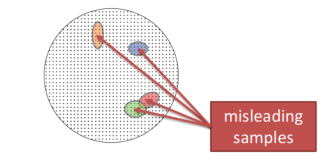
\includegraphics[scale=1.5]{images/misleading_samples.pdf}
\caption{Each point in the large circle represents a possible m-tuple of instances. Each colored oval represents the set of “misleading” m-tuple of instances for some “bad” predictor $h\in\mcl{H}_B$. The $ERM$ can potentially overfit whenever it gets a misleading training set S. That is, for some $h\in\mcl{H}_B$ we have $L_S(h)=0$. The disequations found in the demostration of the theorem guarantee that for each individual bad hypothesis, $h\in\mcl{H}_B$, atmost $(1-\varepsilon)^m$-fraction of the training sets would be misleading. In particular, the larger $m$ is, the smaller each of these colored ovals becomes. The union bound formalizes the fact that the area representing the training sets that are misleading with respect to some $h\in\mcl{H}_B$ (that is, the training sets in M) is atmostthe sum of the areas of the colored ovals. Therefore, it is bounded by $\mcl{H}_B$ times the maximum size of a colored oval. Any sample S outside the colored ovals cannot cause the $ERM$ rule to overfit.}
\end{figure}



\chapter{PAC Learning}

The title of this chapter stands for \textit{Probably Approximately Correct} learning: since the data are sampled accordingly to $\mcl{D}$, and since we can't find the perfect machine learning algorithm:
\begin{itemize} 
\item we can only be approximately correct (accuracy parameter $\varepsilon$: we are satisfied with a good $h_S$ for which $L_{\mcl{D},f}(h_S)\leq\varepsilon$)
\item we can only be probably correct (we want $h_S$ to be a good hypothesis with probability $\geq 1-\delta$)
\end{itemize}

\begin{DEF}
(\textbf{PAC learnability})\\
A hypothesis class $\mcl{H}$ is PAC learnable if there exist a function $m_\mcl{H}:(0,1)^2\to\mathds{N}$ and a learning algorithm such that for every $\delta,\varepsilon\in(0,1)$, for every distribution $\mcl{D}$ over $\mcl{X}$, and for every labeling function $f:\mcl{X}\to\left\{0,1\right\}$, if the realizability assumption holds with respect to $\mcl{H},\mcl{D},f$, then when running the learning algorithm on $m\geq m_\mcl{H}(\varepsilon,\delta)$ i.i.d. examples generated by $\mcl{D}$ and labeled by $f$, the algorithm returns a hypothesis $h$ such that, with probability $\geq 1-\delta$ (over the choice of examples): $\ell_{\mcl{D},f}(h)\leq\varepsilon$.
\label{def:PAC_learn}
\end{DEF}

Note: $m_\mcl{H}:(0,1)^2\to\mathds{N}$ is the sample complexity of learning $\mcl{H}$, in particular is the minimal integer that satisfies the requirements. This means that if we have an infinite number of possible hypotesis we cannot apply the theorem, but, at the same time, we can't be sure that the set is not learnable.\\

\begin{COR}
Every finite (sufficient condition, not necessary, as said before) hypothesis class is PAC learnable with sample complexity
\[ m_\mcl{H}(\varepsilon,\delta)\leq\left[ \frac{\log(\abs{\mcl{H}}/\delta)}{\varepsilon} \right] \]
\end{COR}

The definition of PAC learnability contains two approximation parameters. The accuracy parameter $\varepsilon$
 determines how far the output classifier can be from the optimal one and a confidence parameter $\delta$ indicating how likely the classifier is tomeet that accuracy requirement.\\

\vspace{0.5cm}
Now we would like to generalize this model, and we can do it dropping some assumptions we have made before:
\begin{itemize}
\item We remove the realizability assumption: it was interesting from a theorical point of view but too strong in many real world applications. Rejecting this means that there exist $h^*\in\mcl{H}$ such that $L_{\mcl{D},f}(h)=0$.
\item In many application it is not too realistic that the labeling is fully determined by the features we measure; for this reason it is convenient to replace the function $f$ with something more flexible, for example assuming that $\mcl{D}$ is a probability distribution over $\mcl{X}\times\mcl{Y}$ (i.e. the joint distribution over domain points and labels). One can view such a distribution as being composed of two parts: a distribution $\mcl{D}_x$ over unlabeled domain points (\textit{marginal distribution}) and a \textit{conditional} probability over labels for each domain point $D((x,y)|x)$.
\end{itemize}

\section{The empirical and the true error}
For a probability distribution $\mcl{D}$ over $\mcl{X}\times\mcl{Y}$ we redefine the true error (or risk) of a prediction rule $h$ to be
\begin{equation}
L_\mcl{D}(h) = \mathds{P}_{(x,y)\sim\mcl{D}}[h(x)\neq y] = \mcl{D}([(x,y):h(x)\neq y])
\label{eq:true_err_D}
\end{equation}

Note: in the previous definition \ref{eq:err_pred_rule} the request was $[h(x)\neq f(x)]$ but, as we said before, the function $f(x)$ doesn't exist anymore because it was a too strong assumption asking that the labels were fully determined by a single function.\\
The definition of the empirical risk, instead, remains the same as before
\[ L_S(h)=\frac{[i\in[m]:h(x_i)\neq y_i]}{m} \]
and still represent the probability that, for a pair $(x_i,y_i)$ taken uniformily at random training data, the event "$h(x_i)\neq y_i$" holds.

\section{The Bayes optimal predictor}
Given any probability distribution $\mcl{D}$ over $\mcl{X}\times [0,1]$, the best label predicting function (the one that minimize $L_\mcl{D}(h)$) will be
\begin{equation}
f_\mcl{D}(x) = \left\{\begin{aligned} &1\quad \text{if  } \mathds{P}[y=1|x]\geq 1/2\\ &0\quad \text{otherwise}\end{aligned}\right.
\label{eq:bayes_predictor}
\end{equation}

It's easy to verify that the predictor $f_\mcl{D}$ is optimal, in the sense that any other classifier $g:\mcl{X}\to [0,1]$, has a lower error, $L_\mcl{D}(f_\mcl{D})\leq L_\mcl{D}(g)$.\\
This optimal predictor is interensting from a theorical point of view, but unfortunately is not usable in practice because e don't know the distribution $\mcl{D}$ and, consequently $\mathds{P}[y=1|x]$.\\


\section{Agnostic PAC Learnability}
Clearly, we cannot hope that the learning algorithm will find a hypothesis whose error is smaller than the minimal possible error, that of the Bayes predictor. Furthermore, as we shall prove later, once we make no prior assumptions about the data-generating distribution, no algorithm can be guaranteed to find a predictor that is as good as the Bayes optimal one. Instead, we require that the learning algorithm will find a predictor whose error is not much larger than the best possible error of a predictor in some given benchmark hypothesis class. Of course, the strength of such a requirement depends on the choice of that hypothesis class.\\
\begin{DEF}(\textbf{Agnostic PAC Learnability})\\
A hypothesis class $\mcl{H}$ is agnostic PAC learnable if there exist a function $m_\mcl{H}:(0,1)^2\to\mathds{N}$ and a learning algorithm such that for every $\delta,\varepsilon\in (0,1)$ and for every distribution $\mcl{D}$ over $\mcl{X}\times\mcl{Y}$, when running the algorithm on $m\geq m_\mcl{H}(\varepsilon,\delta)$ i.i.d. examples generated by $\mcl{D}$ the algorithm returns a hypothesis $h$ such that, with probability $\geq 1-\delta$ (over the choice of the $m$ training examples):
\[ L_\mcl{D}(h)\leq\min_{h'\in\mcl{H}}L_\mcl{D}(h')+\varepsilon \]
\label{def:agnostic_PAC_l}
\end{DEF}
Notes on the definition:
\begin{itemize}
\item The agnostic PAC learning generalizes the definition of PAC learning, in the sense that, if the realizability assumption holds, this new definition provides the same guarantee as the previous one.
\item The realizability assumption would implies that the quantity $\min_{h'\in\mcl{H}}L_\mcl{D}(h')$, that represents the performance of the best possible classifier (for example the Bayes' one), is always equal to zero.
\end{itemize}
Anyway a learner can still declare success if its error is not much larger than the best error achievable by a predictor from the class $\mcl{H}$. This is in contrast to PAC learning, in which the learner is required to achieve a small error in absolute terms and not relative to the best error achievable by the hypothesis class.\\ 

\vspace{0.5cm}
We now want to extend our model so that it can be applied to a wide variety of learning tasks. Let's consider 3 different possible problems:
\begin{itemize}
\item \textit{Binary and Multiclass classification}: our training sample will be a finite sequence of (feature vector,label) pairs, the learner’s output will be a function from the domain set to the label set, and, finally, for our measure of success, we can use the probability, over pairs, of the event that our predictor suggests a wrong label.
\item \textit{Regression}: in this task, one wishes to find some simple pattern in the data, a function between $\mcl{X}$ and $\mcl{Y}=\mathds{R}$. For the loss function, we can't use the same of the previous case, we need a new one.
\end{itemize}

\subsection{Generalized loss function}
Given any set $\mcl{H}$ (that plays the role of our hypotheses, or models) and some domain $Z$ let $\ell$ be any function from $\mcl{H}\times Z$ to the set of nonnegative real numbers, $\ell:\mcl{H}\times Z\to\mathds{R}+$. We call such functions loss functions.\\
We now define the \textbf{risk function} to be the expected loss of a classifier $h\in\mcl{H}$, with respect to a probability distribution $\mcl{D}$ over $Z$, namely:
\begin{equation}
L_\mcl{D}(h) = \mathds{E}_{z\sim\mcl{D}}\left[\ell(h,z)\right]
\label{eq:risk_func}
\end{equation}
Similarly, we define the \textbf{empirical risk} to be the expected loss over a given sample $S=(z_1,\dots,z_m)\in Z^m$, namely:
\begin{equation}
L_S(h) = \frac{1}{m}\sum_{i=1}^m\ell(h,z_i)
\label{eq:emp_risk}
\end{equation}

We must keep in mind that the loss always depends on the problem, there isn't a universal one. Sometimes it is useful to create a "personalized" loss function.\\
Common loss functions:
\begin{itemize}
\item \textit{0-1 loss}: commonly use in binary or multiclass classification (obviously is not the only possible solution, is just the simpler and most common one).
\[ \ell_{0-1}(h,(x,y))=\left\{\begin{aligned} &0\quad\text{if  }h(x)=y\\ &1\quad\text{if  }h(x)\neq y\end{aligned}\right. \]
\item \textit{Squared loss L2}: commonly used in regression, penalize few large errors.
\[ \ell_{sq}(h,(x,y))=(h(x)-y)^2 \]
\item \textit{Absolute value loss L1}: commonly used in regression, penalize many small errors:
\[ \ell_{abs}(h,(x,y))=\abs{h(x)-y} \]
\end{itemize}

\begin{EX} The loss function depends on our problem!
Let's image a machine learning algorithm that verify fingerprints to guarantee the access to something. There are essentially two types of error that the computer can do:
\begin{itemize}
\item \textit{False accept}: when accepts an unauthorized user.
\item \textit{False reject}: when doesn't accept an athorized user.
\end{itemize}
If, for example, a supermarket implement the algorithm to give discounts:
\begin{itemize}
\item[-] False reject is costly; just the customer gets annoyed.
\item[-] False accept is minor, the supermarket lose just a discount and the intruder left his fingerprints.
\end{itemize}
If, instead, a similar algorithm has been implemented by CIA for the security of a certain area:
\begin{itemize}
\item[-] False reject can be tolerade.
\item[-] False accept is a disaster!
\end{itemize}
This example want to show that often the loss function need to be "calibrated" by our knowledge on the problem, to understand which errors are tolerable and which are not.
\end{EX}

\begin{DEF} (\textbf{Agnostic PAC Learnability for General Loss Functions})\\
Recalling the definition \ref{def:agnostic_PAC_l}, for which the hypothesis generate by the algorithm (with probability $\geq 1-\delta$ over the training set) has a true error
\[ L_\mcl{D}(h)\leq\min_{h'\in\mcl{H}}L_\mcl{D}(h')+\varepsilon \]
we can implement the definition we have written for the loss function deducing that:
\[ L_\mcl{D}(h) = \mathds{E}_{z\sim\mcl{D}}\left[\ell(h,z)\right] \]
\end{DEF}


\chapter{Learning from Uniform Convergence}

Recall that, given a hypothesis class $\mcl{H}$, the ERM learning paradigm works as follow: upon receiving a training sample S, the learner evaluates the error of each $h\in\mcl{H}$ on the given sample and outputs a member of the class that minimizes this empirical risk. The hope is that an $h$ that minimizes the empirical risk with respect to S is a risk minimizer with respect to the true data probability distribution aswell. For this reason we want that the empirical error is a good approximation of the true error for all the solutions, and not only for the best one ($L_S(h)$ is similar to $L_\mcl{D}(h)$, $\forall\, h$).\\
\begin{DEF} (\bm{$\varepsilon$}\textbf{-representative})\\
A training set S is called $\varepsilon$-representative (with respect to domain Z, hypothesis class $\mcl{H}$, loss function $\ell$ and distribution $\mcl{D}$) if 
\[ \forall h\in\mcl{H} \quad \abs{L_S(h)-L_D(h)}\leq\varepsilon \]
\end{DEF}  

This is a stronger request than previous ones because we do not more focus on the best hypothesis of the class.\\

\begin{THEO}
	Assume that the training set $S$ is $\frac{\varepsilon}{2}$-representative. Then, any output of $ERM_\mcl{H}(S)$ (i.e. any $h_S\,\in\,\underset{h\in\mcl{H}}{argmin}\, L_S(h)$) satisfies:
	\[ L_\mcl{D}(h_S)\leq\min_{h\in\mcl{H}} L_\mcl{D}(h)+\varepsilon  \]
\end{THEO} 
\begin{proof}
	For every $h\in\mcl{H},$
	\[ L_\mcl{D}(h_S)\leq L_S(h_S)+\frac{\varepsilon}{2}\leq L_\mcl{D}(h)+\frac{\varepsilon}{2}+\frac{\varepsilon}{2} = L_\mcl{D}(h) + \varepsilon\]
	where the first and the third inequalities are due to the assumption that $S$ is $\frac{\varepsilon}{2}$- and the second inequality holds since $h_S$ is an ERM predictor. 
\end{proof}

The relation guarantee by the theorem is exactly the one required by the definition of agnostic PAC learnability: in fact, the consequence of this statement is that if, with probability at least $1-\delta$, a random training set $S$ is $\varepsilon$-representative, then the ERM rule is an agnostic PAC learner.

\begin{DEF} (\textbf{Uniform Convergence})\\
	A hypothesis class $\mcl{H}$ has the uniform (same $m$ for all $h$ and all $\mcl{D}$) convergence property (with respect to a domain $Z$ and a loss function $\ell$) if there exists a function $m_\mcl{H}^{UC}:(0,1)^2\to\mathds{N}$ such that for every $\varepsilon,\delta\in(0,1)$ and for every probability distribution $\mcl{D}$ over $Z$, if $S$ is a sample of $m\geq m_\mcl{H}^{UC}(\varepsilon,\delta)$ i.i.d. examples drawn from $\mcl{D}$, then with probability $\geq 1-\delta$, $S$ is $\varepsilon$-representative.
\end{DEF} 

This means that the function $m_\mcl{H}^{UC}$ measures the (minimal) sample complexity of obtaining the uniform convergence property, namely, how many examples we need to ensure that with probability at least $1-\delta$ the sample would be $\varepsilon$-representative.

\begin{PROP}
	If a class $\mcl{H}$ has the uniform convergence property with a function $m_\mcl{H}^{UC}$ then the class is agnostically PAC learnable with the sample complexity $m_\mcl{H}(\varepsilon,\delta)\leq m_\mcl{H}^{UC}(\varepsilon/2,\delta)$. Furthermore, in that case the $ERM_\mcl{H}$ paradigm is a successful agnostic PAC learner for $\mcl{H}$.	
\end{PROP}

\begin{PROP}
	Let $\mcl{H}$ be a finite hypothesis class, let $Z$ be a domain, and let $\ell:\mcl{H}\times Z\to[0,1]$ be a loss function. Then:
	\begin{itemize}
		\item $\mcl{H}$ enjoys the uniform convergence property with sample complexity 
		\[ m_\mcl{H}^{UC}(\varepsilon,\delta)\leq\left[\frac{\log(2\abs{\mcl{H}}/\delta)}{2\varepsilon^2}\right] \]
	\item $\mcl{H}$ is agnostically PAC learnable using the ERM algorithm with sample complexity
	\[ m_\mcl{H}(\varepsilon,\delta)\leq m_\mcl{H}^{UC}(\varepsilon/2,\delta)\leq\left[\frac{2\log(2\abs{\mcl{H}}/\delta)}{\varepsilon^2}\right] \]
	\end{itemize}
\end{PROP}
\begin{proof}
	RICORDARSI DI FARE PURE QUESTA 
%%%%%%%%%%%%%%%%%%%%%%%%%%%%%%%%%
\end{proof}

\subsection{The Discretization Trick}
While the previous theorem only applies on finite hypothesis classes, there is a simple trick that allow us to get a very good estimate of the practical sample complexity of infinite hypothesis classes. In many real world application, in fact, we consider classes determined by a set of parameters in $\mathds{R}$.\\
The solution arises when we use computers. Using a pc, in fact, we will probably maintain real numbers using floating point representation, say, of 64 bits. It follows that, in practice, our hypothesis class is parameterized by the set of scalar that can be represented using a 64 bits floating point number. There are at most $2^{64}$ such numbers; hence the actual size of our hypothesis class is at most $2^{64}$. More generally, if our hypothesis class is parameterized by $d$ numbers, in practice we learn an hypothesis class of size at most $2^{64d}$.\\
Applying the proposition, we obtain that the sample complexity of such classes is bounded by
\[ m_\mcl{H}(\varepsilon,\delta)\leq m_\mcl{H}^{UC}(\varepsilon/2,\delta)\leq \frac{2\log\left(2\frac{2^{64d}}{\delta}\right)}{\varepsilon^2} \] 
This upper bound on the sample complexity has the deficiency of being dependent on the specific representation of real numbers used by our machine.


\chapter{The Bias-Complexity Trade-Off}
In one of the previous chapters we saw that, unless one is careful, the training data can mislead the learner, and result in overfitting. To overcome this problem, we restricted the search space to some hypothesis class $\mcl{H}$. Such an hypothesis class can be viewed as reflecting some prior knowledge that the learner has about the task – a belief that one of the members of the class $\mcl{H}$ is a low-error model for the task.\\
Our main objective was, given a training set $S$ and a loss function, to find a function $\hat{h}$ for which the error $L_\mcl{D}(\hat{h})$ is small (that brought to the definition of Agnostic PAC learnability (\ref{def:agnostic_PAC_l})). For this reason we needed a large hypothesis class to contain the best solution, but at the same time a good algorithm to find it.\\
But, is there some kind of universal learner, that is, a learner who has no prior knowledge about a certain task and is ready to be challenged by any task, that predicts the best $\hat{h}$ for any distribution $\mcl{D}$?\\
So, what about using the set of \textit{all} the functions from $\mcl{X}$ to $\mcl{Y}$ as the hypothesis class? With this assumption we would be sure that the solution (if the problem is solvable) is inside the class.\\

\begin{THEO} (\textbf{No-Free Lunch})\\
	Let $A$ be a learning algorithm for the task of binary classification with respect to the 0-1 loss over a domain $\mcl{X}$. Let $m$ be any number smaller than $\abs{\mcl{X}}/2$, representing a training set size. Then, there exists a distribution $\mcl{D}$ over $\mcl{X}\times\left\{0,1\right\}$ such that:
	\begin{itemize}
		\item there exists a function $f:\mcl{X}\to\left\{0,1\right\}$ with $L_\mcl{D}(f)=0$ (so a perfect solution with 0 loss)
		\item with probability of at least $1/7$ over the choice $S\sim\mcl{D}^m$ we have that $L_\mcl{D}(A(S))\geq 1/8$.
	\end{itemize}
\end{THEO} 
This means that there isn't a universal learner: the algorithm can fail even if there is a perfect solution for the training set. In fact, the theorem guarantees the existance of this perfect solution (with 0 loss), but doesn't guarantee a good performance instead.\\
The key message is that for every ML algorithm there exist a task on which it fails even if another ML algorithm is able to solve it.\\

\vspace{0.3cm}
\textit{Idea of the proof}: our training set is smaller than half of the domain. This means that we have no information on what happens on the other half, but we can suppose that there is some target function f that works on the other half in a way that contradicts our estimated labels.\\

\vspace{0.5cm}
Let's consider an ERM predictor over the hypothesis class of all the functions $f:\mcl{X}\to\left\{0,1\right\}$. This class represent a lack of knowledge: every possible function is considered a good candidate. According to the previous theorem, any algorithm that chooses its output from an hypothesis belonging to that class, and in particular the ERM predictor, will fail on some learning task. Therefore, the class is not PAC learnable, as formalized in the following corollary.\\
\begin{COR}
	Let $\mcl{X}$ be an infinite domain set and let $\mcl{H}$ be the set of all the functions from $\mcl{X}$ to $\left\{0,1\right\}$. Then, $\mcl{H}$ is not PAC learnable.
\end{COR}

\begin{proof}
	Let's assume, by way of contradiction, that the class is learnable and let's choose some $\varepsilon <1/8$ and $\delta <1/7$. By the definition of PAC learnability (\ref{def:PAC_learn}), it exists an algorithm $A$ and an integer $m=m(\varepsilon,\delta)$, such that for any data-generating distribution over $\mcl{X}\times\left\{0,1\right\}$, if for some function $f$ in that domain, $L_\mcl{D}(f)=0$, then with probability $\geq 1-\delta$ when $A$ is applied to samples $S$ of size $m$, generated i.i.d. by $\mcl{D}$, $L_\mcl{D}(A(S))\leq\varepsilon$.\\
	However, applying the Free-Lunch theorem, since $\abs{\mcl{X}}>2m$, for every learning algorithm (and in particular for $A$), there exists a distribution $\mcl{D}$ such that with probability greater than $1/7 >\delta$, $L_\mcl{D}(A(S)) >1/8 >\varepsilon$, which leads to the desired contradiction.
\end{proof}

But how can we prevent such failures? We should, for example, use our knowledge on a specific learning task to avoid distributions that will cause us to fail.\\
But how should we choose a good hypothesis class? On the other hand we want to believe that this class includes the hypothesis that has no error at all (in the PAC setting), or at least that the smallest error achievable by a hypothesis from this class is indeed rather small (in the agnostic setting). On the other hand, we have just seen that we cannot simply choose the richest class i.e. the class of all functions over the given domain.\\
\begin{itemize}
	\item If we choose a \textit{small} $\mcl{H}$ we will deal with \textit{low approximation capabilities} (large $L_S$) but \textit{good generalization properties} ($L_\mcl{D}\sim L_S$). So the approximation found will work similarly on real data as on the training set, but it's not guarantee that the best hypothesis is in the class.
	\item If we choose a \textit{large} $\mcl{H}$, instead, we will have \textit{good approximation capabilities} (small $L_S$) but there is a bigger \textit{risk of overfitting} ($L_\mcl{D}\gg L_S$). Moreover the no free lunch theorem suggests to not have too larger hypothesis classes.
\end{itemize}

\section{Error Decomposition}
To answer these questions we decompose the true error of an $ERM_\mcl{H}$ predictor, $h_S$ into two components, as follows:
\[ L_\mcl{D}(h_S)=\varepsilon_{app}+\varepsilon_{est} \]

\begin{itemize}
	\item \textbf{Approximation error}
	\[ \varepsilon_{app}=\min_{h\in\mcl{H}} L_\mcl{D}(h) \]
	It is the minimum risk achievable by a predictor in the hypothesis class. It does not depend on the training set, or on the sample size, but only on the choice of the class. Enlarging the hypothesis class can decrease the approximation error. Under the realizability assumption, this error is zero.
	\item \textbf{Estimation error}
	\[ \varepsilon_{est} = L_\mcl{D}(h_S) - \min_{h\in\mcl{H}}(h) \]
	It is the difference between the approximation error and the error achieved by the ERM predictor. The estimation error results because the training error is only an estimate of the true risk, and so the predictor minimizing the empirical risk is only an estimate of the predictor minimizing the true risk. This type of error depends on the training set size and on the size, or complexity, of the hypothesis class. For a finite class, the estimation error increases (logarithmically) with $\abs{\mcl{H}}$ and decreases with $m$ (so the training error becomes a good estimate of the true error).
\end{itemize}

The following pictures schematized what we just said regarding the two types of error.

\begin{figure}[!h]
	\centering
	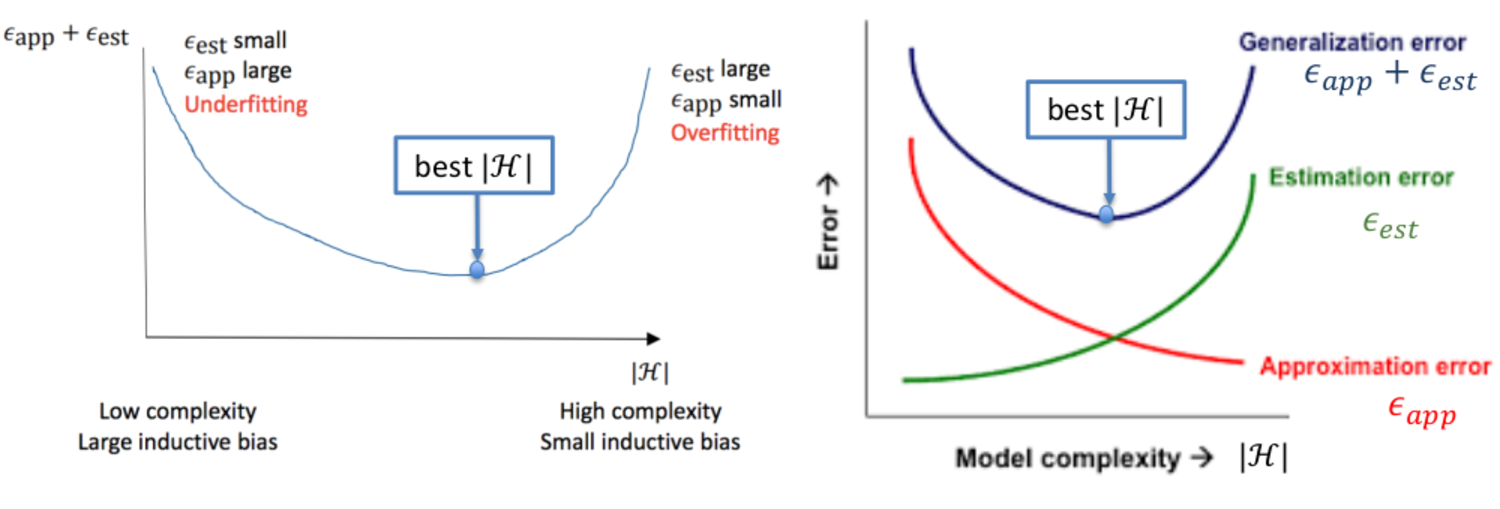
\includegraphics[scale=0.5]{images/error_decomposition.pdf}
	\caption{Error decomposition}
	\label{fig:err_dec}
\end{figure}

Since our goal is to minimize the total risk, we face a \textit{tradeoff}, called the \textbf{bias complexity tradeoff}. On one hand, choosing $\mcl{H}$ to be a very rich class decreases the approximation error but at the same time might increase the estimation error, as a rich $\mcl{H}$ might lead to \textit{overfitting}. On the other hand, choosing $\mcl{H}$ to be a very small set reduces the estimation error but might increase the approximation error or, in other words, might lead to \textit{underfitting}.\\
The differences between overfitting and underfitting can be seen in picture \ref{fig:under_over_fit}.\\

\begin{figure}[!h]
	\centering
	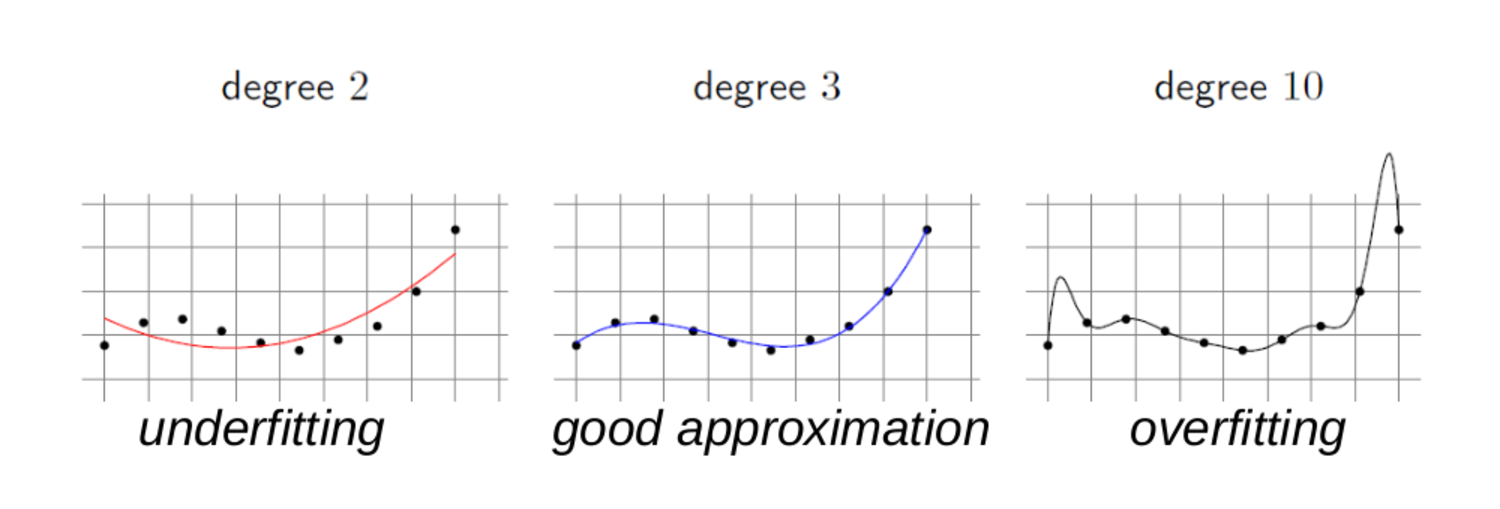
\includegraphics[scale=0.7]{images/over_under_fitting.pdf}
	\caption{Comparison between underfitting and overtitting}
	\label{fig:under_over_fit}
\end{figure}

\vspace{0.5cm}
We need to estimate the generalization error $L_\mcl{D}(h)$ for a function h (the one selected with ERM). To do this, we use a \textit{test set}, a new set of samples different (disjoint) from the training set used to pick h. Sometimes we use also a \textit{validation set} for selecting the hyper-parameters of the algorithm or to evaluate errors while iterative training procedures are running.\\
To summarize the procedure of training a ML algorithm parametrized by some Hyper-Parameters (HP):
\begin{itemize}
	\item[1.] Select Hyper-Parameters values
	\item[2.] Train the algorithm with the choosen parameters on the training set
	\item[3.] Evaluate performances on the validation set
	\item[4.] Go back to 1. and select new HP values
	\item[5.] Select the final HP leading to the smallest validation error
	\item[6.] Compute error estimation on the test set  
\end{itemize}


\chapter{Linear Predictors}

\chapter{VC Dimension}
We have seen, in the previous chapters, that a finite class ($\abs{\mcl{H}}<\infty$) is agnostic PAC learnable. What about infinite classes? We would like to understand when infinite classes are learnable and also the number of samples that we need to work with.\\ To show that the size of the hypothesis class is not the right characterization of its sample complexity, we first present a simple example of an infinite-size hypothesis class that is learnable.\\

\vspace{0.5cm}
\begin{EX}
	Let $\mcl{H}$ be the set of \textit{threshold functions} over the real line, namely $\mcl{H}=\left\{h_a:a\in\mathds{R}\right\}$ where $h_a:\mathds{R}\to\left\{0,1\right\}$ is a function such that $\left\{\begin{aligned}&1\quad\text{if}\quad x<a\\&0\quad\text{otherwise}\end{aligned}\right.$.\\
	Clearly, $\mcl{H}$ is of infinite size, but we can show that $\mcl{H}$ is PAC learnable, using the ERM rule, with sample complexity $m_\mcl{H}(\varepsilon,\delta)\leq\left[\log(2/\delta)/\varepsilon\right]$.
	
	\begin{proof}
		Let $a^*$ be a threshold such that the hypothesis $h^*(x)$ achieves $L_\mcl{D}(h^*)=0$. Let $\mcl{D}_x$ be the marginal distribution over the domain $\mcl{X}$ and let $a_0 < a^* < a_1$ be such that
		\[ \underset{x\sim\mcl{D}_x}{\mathds{P}}\left[x\in(a_0,a^*)\right]= \underset{x\sim\mcl{D}_x}{\mathds{P}}\left[x\in(a^*,a_1)\right]=\varepsilon \]
		Given a training set S, let $b_0=\max\left\{x:(x,1)\in S\right\}$ and $b_1=\min\left\{x:(x,0)\in S\right\}$. Let $b_S$ be a threshold corresponding to ERM hypothesis $h_S$, which implies that $b_S\in(b_0,b_1)$. Therefore, the sufficient condition for $L_\mcl{D}(h_S)\leq\varepsilon$ is that both $b_0\geq a_0$ and $b_1\leq a_1$. In other words):
		\[ \underset{S\sim\mcl{D}^m}{\mathds{P}}\left[L_\mcl{D}(h_S)>\varepsilon\right]\leq \underset{S\sim\mcl{D}^m}{\mathds{P}}\left[b_0<a_0\vee b_1>a_1 \right] \leq\underset{S\sim\mcl{D}^m}{\mathds{P}}\left[b_0<a_0\right]+\leq\underset{S\sim\mcl{D}^m}{\mathds{P}}\left[b_1>a_1\right] \]
		where, in the second disequation, we used the union bound. 
		The event $b_0<a_0$ happens only if all examples in S are not in the interval $(a_0,a^*)$, whose probability mass is defined to be $\varepsilon$, namely:
		\[ \underset{S\sim\mcl{D}^m}{\mathds{P}}\left[b_0<a_0\right]=\leq\underset{S\sim\mcl{D}^m}{\mathds{P}}\left[\forall (x,y)\in S,\; x\notin(a_0,a^*)\right] = (1-\varepsilon)^m \leq e^{-\varepsilon m} \]
		Since we assume $m\geq \log(2/\delta)/\varepsilon$ it follows that the equation is at most $\delta/2$. In the same way it is easy to see that 
		\[ \underset{S\sim\mcl{D}^m}{\mathds{P}}\left[b_1>a_1\right]\leq \frac{\delta}{2} \]
		Combining it with the previous relation we conclude our proof.	
	\end{proof}
\end{EX}
\vspace{0.5cm}

We see, therefore, that while finiteness of $\mcl{H}$ is a sufficient condition for learnability, it is not a necessary condition.\\
Before giving the next definitions, let us recall the No Free Lunch theorem and its proof: we have shown that without restricting the hypothesis class, for any learning algorithm, an adversary can construct a distribution for which the learning algorithm will perform poorly, while there is another learning algorithm that will succeed on the same distribution. To proove that, the idea was to select a distribution concentrated on a set C (so a restriction) on which the algorithm fails. Since we are considering distributions that are concentrated on elements of C, we should study $\mcl{H}$ behaves on C.
\begin{DEF}(\textbf{Restriction of $\mcl{H}$ to C})\\
	Let $\mcl{H}$ be a class of functions from $\mcl{X}$ to $\left\{0,1\right\}$ and let $C=\left\{c_1,\dots ,c_m\right\}\subset\mcl{X}$. The restriction $\mcl{H}_C$ of $\mcl{H}$ to C is:
	\[ \mcl{H}_C=\left\{\left[h(c_1),\dots ,h(c_m)\right] :h\in\mcl{H}\right\} \]
	where we represent each function from C to $\left\{0,1\right\}$ as a vector in $\left\{0,1\right\}^\abs{C}$.
\end{DEF}
If the restriction of $\mcl{H}$ in C is the set of all functions from C to $\left\{0,1\right\}$, then we say that $\mcl{H}$ \textit{shatters} the set C. Formally
\begin{DEF}(\textbf{Shattering})\\
	A hypothesis class $\mcl{H}$ shatters a finite set $C\subset\mcl{X}$ if the restriction of $\mcl{H}$ to C is the set of all functions from C to $\left\{0,1\right\}$, that is $\abs{\mcl{H}_C} =2^\abs{C}$.
\end{DEF}
Getting back to the construction of an adversarial distribution as in the proof of the No-Free-Lunch theorem, we see that whenever some set C is shattered by $\mcl{H}$, the adversary is not restricted by $\mcl{H}$, as they can construct a distribution over C based on any target function from C to $\left\{0,1\right\}$, while still maintaining the realizability assumption. This immediately yields:
\begin{COR}
	Let $\mcl{H}$ be a hypothesis class of functions from $\mcl{X}$ to $\left\{0,1\right\}$. Let $m$ be a training set size. Assume that there exist a set $C\subset\mcl{X}$ of size $2m$ that is shattered by $\mcl{H}$. Then for any learning algorithm A there exist a distribution $\mcl{D}$ over $\mcl{X}\times\left\{0,1\right\}$ and a predictor $h\in\mcl{H}$ such that $L_d(h)=0$ but with probability at least 1/7 over the choice of S we have that $L_\mcl{D}(A(S))\geq 1/8$.
	\label{cor:NFL_shattering}
\end{COR}
This corollary tells us that if $\mcl{H}$ shatters some set C of size $2m$ then we cannot learn $\mcl{H}$ using $m$ examples.
\begin{DEF}(\textbf{VC-dimension})\\
	The VC-dimension of an hypothesis class $\mcl{H}$, denoted $VCdim(\mcl{H})$, is the maximal size of a set $C\subset\mcl{X}$ that can be shattered by $\mcl{H}$. If $\mcl{H}$ can shatter sets of arbitrarily large size we say that $\mcl{H}$ has infinite VC-dimension.
\end{DEF}

Notice that:
\begin{itemize}
	\item If $\mcl{H}$ is a finite class, for any set $C$ we have $\abs{\mcl{H}_C}\leq\abs{H}$ and thus C cannot be shattered if $\abs{\mcl{H}}\leq2^\abs{C}$. This implies that $VCdim(\mcl{H})\leq\log_2(\abs{\mcl{H}})$.
	\item If $\mcl{H}$ has an infinite VC-dimension it is not PAC learnable: as a consequence of the corollary \ref{cor:NFL_shattering}, there will always exist a subset of size $2m$ that is shattered for any $m$.
\end{itemize}

To show that $VCdim(\mcl{H})=d$ we need to show that:
\begin{itemize}
	\item[1.] $VCdim(\mcl{H})\geq d$: there exists a set $C$ of size $d$ that is shattered by $\mcl{H}$.
	\item[2.] $VCdim(\mcl{H})\leq (d+1)$: every set $C$ of size $d+1$ is not shattered by $\mcl{H}$.
\end{itemize}

\begin{EX} (Threshold functions)\\
	Let $\mcl{H}$ be the class of threshold functions over $\mathds{R}$. Take a set $C=\left\{c_1\right\}$. Now, if we take $a=c_1+1$, then we have $h_a(c_1)=1$, and if we take $a=c_1-1$, then we have $h_a(c_1)=0$. Therefore, $\mcl{H}_C$ is the set of all the functions from $C$ to $\left\{0,1\right\}$, and $\mcl{H}$ shatters $C$. Now let's take a set $C=\left\{c_1,c_2\right\}$, where $c_1\leq c_2$. No $h\in\mcl{H}$ can account for the labeling $(0,1)$, because any threshold that assign the label 0 to $c_1$ must assign the label 0 to $c_2$ as well. Therefore not all functions from $C$ to $\left\{0,1\right\}$ are included in $\mcl{H}_C$; hence $C$ is not shattered by $\mcl{H}$.\\
	So, we just proved that an arbitrary set $C=\left\{c_1\right\}$ is shattered by $\mcl{H}$ (where $\mcl{H}$ is the class of threshold functions over $\mathds{R}$); therefore $VCdim(\mcl{H})\geq 1$. At the same time, an arbitrary set $C=\left\{c_1,c_2\right\}$ is not shattered by $\mcl{H}$. So we can conclude that $VCdim(\mcl{H})=1$.
\end{EX}

\begin{EX} (Intervals)\\
	Let $\mcl{H}$ be the class of intervals over $\mathds{R}$, namely $\mcl{H}=\left\{h_{a,b}:a,b\in\mathds{R},a<b\right\}$, where $h_{a,b}:\mathds{R}\to\left\{0,1\right\}$ is a functions that is 1 for $x\in(a,b)$ and 0 otherwise. Let's take the set $C=\left\{1,2\right\}$. Then, $\mcl{H}$ shatters $C$ and therefore $VCdim(\mcl{H})\geq 2$. Now let's make an arbitrary set $C=\left\{c_1,c_2,c_3\right\}$ and assume without loss of generality that $c_1\leq c_2\leq c_3$. Then, the labeling (1,0,1) cannot be obtained by an interval, and therefore $\mcl{H}$ does not shatter $C$. We therefore conclude that $VCdim(\mcl{H})=2$.
\end{EX}

\begin{EX} (Axis aligned rectangles)\\
	Let $\mcl{H}$ be the class of axis aligned rectangles, formally: $\mcl{H}=\left\{h_{(a_1,a_2,b_1,b_2)}:a_1\leq a_2 \text{ and } b_1\leq b_2 \right\}$, where 
	\[ h_{(a_1,a_2,b_1,b_2)} = \left\{\begin{aligned}&1\quad if\; a_1\leq x_1\leq a_2 \text{ and } b_1\leq x_2\leq b_2\\ &0\quad\text{otherwise}\end{aligned}\right. \]
	
	As can be seen in figure \ref{fig:axis_al_rect}, it is easy to find a set of 4 points that are shattered, so $VCdim(\mcl{H})\geq 4$. 
	\begin{figure}[!h]
		\centering
		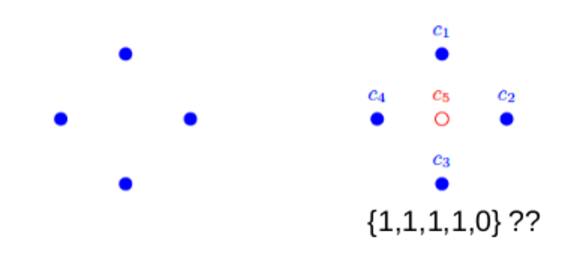
\includegraphics[scale=1]{images/axis_aligned_rectangles.pdf}
		\caption{Left: 4 points are shattered by axis aligned rectangles. Right: any axis aligned rectangle cannot label $c_5$ by 0 and the rest of the points by 1}
		\label{fig:axis_al_rect}
	\end{figure}
	Now let's consider any set $C\in\mathds{R}^2$ of 5 points from which we are gonna take the leftmost, the rightmost, the highest and the lowest one. Without loss of generality, denote $C=\left\{c_1,\dots,c_5\right\}$ and let $c_5$ be the point that was not selected. It is impossible to obtain the label (1,1,1,1,0) by any axis aligned rectangle, because such rectangle must contain $c_1,\dots,c_4$, but at the same time must contain $c_5$ too, because its coordinates are within the intervals defined by the selected points. So this $C$ is not shattered by $\mcl{H}$, and therefore $VCdim(\mcl{H})=4$.
\end{EX}
















\end{flushleft}
\end{document}
